% !TEX encoding = UTF-8
% !TEX TS-program = pdflatex
% !TEX root = ../tesi.tex

%**************************************************************
\chapter{Technologies}
\label{cap:technologies}
\intro{This chapter discusses the technologies \textbf{used} or \textbf{considered} during the project, providing an in-depth description and motivating their choice.}

\section{Docker}
Docker is defined as a set of platform as a service (PaaS$_G$) products that use OS$_G$-level virtualization to package and run applications in loosely isolated environments called \textit{containers} \cite{site:docker-wiki}. \\
These containers can be seen as lightweight virtual machines, containing all the software needed to run applications. The flexibility of such environments makes it easy to run multiple simultaneous instances of them on the same host, allocating them a defined quantity of resources. \\ \\
In general, the main features of Docker are \cite{site:docker-website}:
\begin{itemize}
	\item \textit{contained environments}: considering the isolation provided by Docker containers, its possible atomically perform changes to the software that is being hosted, without impacting any component outside of that environment;
	\item \textit{responsive deployment and scaling}: Docker's lightweight nature makes it possible to dynamically manage workloads, scaling up or tearing down applications and services as needed, in real time;
	\item \textit{running more workloads on the same hardware}: Docker containers require much less computational resources to manage, with respect to complete hypervisor-based virtual machines;
	\item \textit{inter-container communication}: despite being isolated, it is possible for applications running inside Docker containers to interact with each other, if they are configured with the same Docker network.
\end{itemize}
If we compare these characteristics with the needs of Game Engine modules in a distributed architecture, it is easy to see them matching reasonably well with each other. Thus we can consider Docker as an interesting alternative for the implementation of Distributed Game Engine modules.

\subsection{Architecture}
Docker is designed with a client-server architecture \cite{site:docker-overview}, composed of:
\begin{itemize}
	\item \textit{Docker client}: which talks to a daemon and it's one of the primary ways to interact with Docker;
	\item \textit{Docker daemon}: which performs the operations related to building, running and distributing Docker containers.
\end{itemize}
Both these components can be run on the same system or remotely, communicating using REST API$_G$ and using UNIX sockets or a dedicated network interface.
\begin{figure}[h!]
	\centering
	\includegraphics[width=1\linewidth]{"immagini/Technologies/Docker architecture"}
	\caption[Representation of the Docker architecture.]{Representation of the Docker architecture.}
	\label{fig:docker-architecture}
\end{figure}


\subsection{Docker-compose}\label{docker-compose}
Compose is a tool used for defining and running applications which require multiple Docker containers, in a simplified manner \cite{site:docker-compose-doc}. Using Compose, it's possible to provide a single YAML$_G$ file to configure the services needed by the application and then, with a single command, create and start all these containerized services. \\
Some of the main features provided by this tool are:
\begin{itemize}
	\item \textit{multiple isolated environments on a single host}, which, even if possible without this tool, is made much easier and configurable;
	\item \textit{preservation of volume data}, useful for applications that needs to be restated multiple times;
	\item \textit{only recreates containers that have changed}, removing unnecessary build time from the application development process;
	\item \textit{support for environment variables}, very important for correctly configuring software which interacts with the hardware (e.g. X11).
\end{itemize}
Overall, this tool can prove quite helpful when developing distributed systems using Docker.

\subsection{Nvidia-docker}
The NVIDIA Container Toolkit allows users to build and run GPU accelerated Docker containers. The toolkit comprises both a container runtime library and utilities to automatically configure containers to leverage NVIDIA GPUs \cite{site:nvidia-docker-doc}. \\ \\
The main components \cite{site:nvidia-docker-repo} include:
\begin{itemize}
	\item the \texttt{nvidia-docker} wrapper;
	\item the \textit{NVIDIA Container Runtime}, which mostly includes NVIDIA specific code and additional hooks;
	\item the\textit{ NVIDIA Container Runtime Hook}, which includes a script that implements the interface required for the start-up of the container and settings of configurations;
	\item the \textit{NVIDIA Container Library and CLI$_G$}, providing a library and a simple CLI$_G$ utility to configure GNU/Linux containers leveraging NVIDIA GPUS.
\end{itemize}
\begin{figure}[h!]
	\centering
	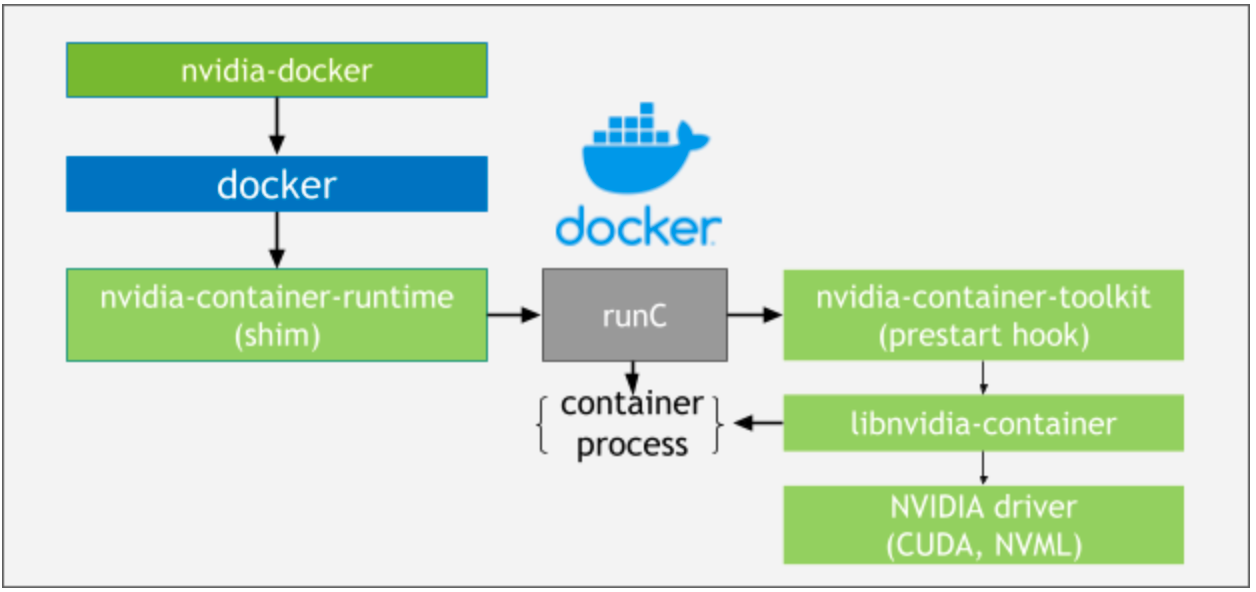
\includegraphics[width=0.9\linewidth]{immagini/Technologies/nvidia-docker-arch-new}
	\caption[Nvidia-docker architecture.]{Nvidia-docker architecture.}
	\label{fig:nvidia-docker-arch-new}
\end{figure}
This toolkit can be an interesting addition for implementing Game Engine graphics modules. However, it is currently not compatible with Docker-compose, which is also an important tool for building distributed system applications.

\section{ETCD}
ETCD is described as a disk-based, distributed and reliable Key-Value Store, which allows the storage of data that can be accessed by a distributed system \cite{site:etcd-desc}. More specifically, ETCD is designed to reliably store infrequently updated data, exposing previous versions of key-value pairs to support inexpensive snapshots of the DB$_G$ and watch history events \cite{site:etcd-data-model}. \\ \\
In order to provide these features, ETCD presents a persistent, multi-version, concurrency-control data model for its key-value storage. This component preserves the previous version of any key-value pair when its value is overwritten with new data. As such, this storage system is described as immutable, since its operations do ot update the structure in-place, but instead generate a new updated structure, where all past versions of the keys are accessible and watchable after modification. \\ \\
In order to guarantee the storage of strongly consistent data, ETCD uses a leader-based consensus protocol called \textit{Raft} for data replication and log execution. The implementation of such algorithm, as well as the rest of ETCD architecture, is developed in the Go programming language, which is particularly fitting for distributed system environments.

\subsection{The Raft Algorithm}
The Raft algorithm is typically adopted in the context of \textit{state machine replication (SMR)} \cite{site:state-machine-replication-wiki}, which is a general method for implementing a fault-tolerant service. This is done by replicating servers (or nodes) and coordinating client interactions with the server replicas. \\
The state machine can be defined as a combination of:
\begin{itemize}
	\item a set of \textit{states};
	\item a set of \textit{inputs};
	\item a set of \textit{outputs};
	\item a transition function, described as: $input \times state \rightarrow state$; 
	\item an output function, described as: $input \times state \rightarrow output$;
	\item a specific \textit{state} called \textit{start};
\end{itemize}
The maximum number of machine replicas that can fail, while still keeping the system operating, is defined by the \textit{crash-fault tolerance}. Moreover, the state machine is required to be \textit{deterministic}, which means that its replicas, starting from the same state and receiving the same input, should return the same output. \\ \\
In this context, a consensus algorithm is required in order to determine and preserve the only authoritative version of the command execution history, in a strongly consistent log.
\begin{figure}[h!]
	\centering
	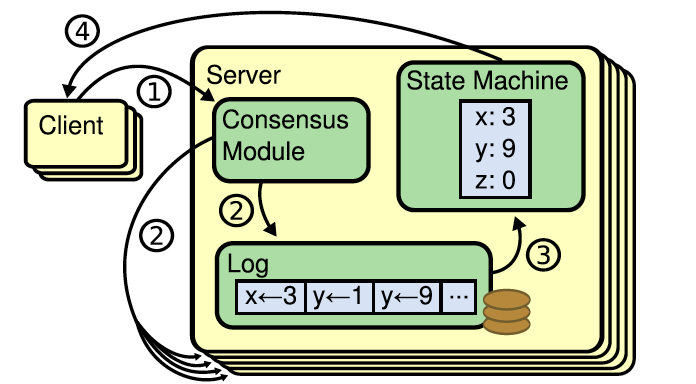
\includegraphics[width=0.7\linewidth]{"immagini/Technologies/image5.png"}
	\caption{Replicated state machine interactions.}
	\label{fig:states}
\end{figure}
\subsubsection{Algorithm overview}
The main goal of the Raft algorithm is to allow distributed nodes to achieve \textit{consensus} on the system state. This means that multiple servers or nodes must agree on some data value that is needed during computation \cite{site:consensus-wiki, site:raft-consensus-algorithm}. This is, generally, a primary objective in the design of fault-tolerant distributed systems. \\ \\
The Raft algorithms defines three main roles, which may be assumed by any node in certain specific situations:
\begin{itemize}
	\item \textit{Follower}: which is a simple node that composes the replicated state machine. This is the default role assigned to nodes when they become part of the \textit{server cluster}, which we define as the subset of nodes that implements the Raft algorithm in a distributed system. Follower nodes may only respond to Candidate and Leader nodes;
	\item \textit{Candidate}: which is a node competing with other Candidate nodes to assume the role of Leader of the distributed system. Nodes may assume this role to request a Leader election, in a situation in which the current Leader node is unresponsive;
	\item \textit{Leader}: which is unique and the only node that interacts with the client. Any request made to Follower nodes is redirected to the Leader node.
\end{itemize}
As previously mentioned, these roles are very important for Raft to be implemented for asymmetric multi-server distributed systems.
\begin{figure}[h]
	\centering
	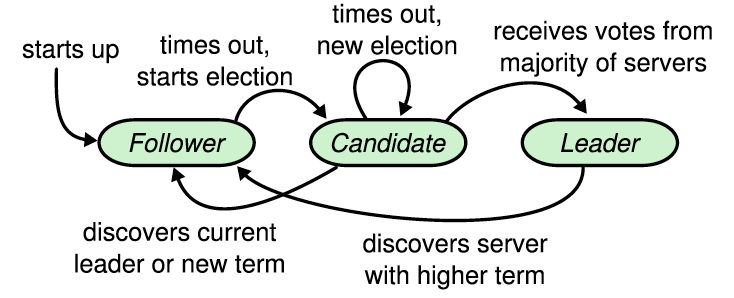
\includegraphics[width=0.7\linewidth]{"immagini/Technologies/image3.png"}
	\caption{Representation of the Raft roles.}
	\label{fig:roles}
\end{figure}
\subsubsection{Time management}
In order to correctly handle server states, the Raft algorithm manages the time by dividing it in \textit{terms} \cite{site:raft-consensus-algorithm}. \\
Working in an asynchronous environment, these terms are not identified by a fixed real-time length. Different servers may observe the transition between terms at different times, while the most significant element of reference is actually the local state of each server. As such, the terms are meant to act as a logical clock, allowing servers to detect obsolete information and stale Leaders, regardless of the asynchronous nature of the system. \\ \\
Each term is uniquely identified by a monotonically increasing integer number called \textit{term number}. This number is stored in each node and attached in node communications. \\
Each term starts with a Leader election, where the Candidates request votes to other server nodes (Followers) in order to obtain a majority consensus:
\begin{itemize}
	\item if a Candidate node manages to obtain the majority of the votes, that Candidate becomes the Leader for the current term;
	\item if no Candidate node manages to obtain the majority of the votes, this situation is called \textit{split vote} and the term will conclude with no elected Leader.
\end{itemize}
As such, a term can only have one single Leader at any time. Moreover, the term number is also a very important indicator for various system tasks, such as:
\begin{itemize}
	\item \textit{term number update}: if a node term number is lower than the one of the other nodes in the cluster, it will be updated at the beginning of a new term. The term numbers used for reference are the ones of the Candidates and the one of the Leader, which usually takes the priority;
	\item \textit{role demotion}: if a Candidate or Leader term number is lower than the other nodes in the cluster, they are demoted to Followers;
	\item \textit{node communication}: the term number of a node is sent as an attachment to each request they make to other nodes. If a request is made with an outdated term number, it is always discarded.
\end{itemize}
This makes the term number a crucial factor in time management, for the Raft algorithm.

\begin{figure}[h]
	\centering
	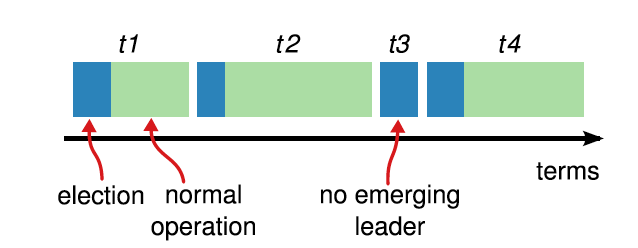
\includegraphics[width=0.7\linewidth]{"immagini/Technologies/image2.png"}
	\caption{Representation of terms (\textit{t\#}).}
	\label{fig:terms}
\end{figure}
\subsubsection{Leader election}
In order to maintain the authority as Leader of the cluster, the node sends periodic messages to the other Follower nodes. These communications are called \textit{heartbeats} \cite{site:raft-consensus-algorithm}. \\ \\
When a Follower node doesn't receive a heartbeat within a given time bound, it assumes the Leader is not active anymore and promotes itself to the role of Candidate. It then votes for itself and requests other nodes to vote for itself, in order to establish a majority. The result of the election can be one of:
\begin{itemize}
	\item the Candidate node receives a vote from the majority of the nodes of the cluster, making it the new Leader. In that moment, the node begins to send heartbeats to notify other nodes of the presence of a new Leader. Candidate nodes receiving the heartbeat will return to the Follower role;
	\item the Candidate node does not manage to get votes from the majority of the nodes of the cluster. In this case, the election ends with no Leader and the node returns to the Follower role;
	\item if the term number of the Candidate node who requested the votes is lower than other Candidate nodes in the cluster, the request is immediately refused and the other nodes keep their Candidate role.
\end{itemize}
This whole process is performed multiple times during the Raft algorithm lifecycle in distributed systems. It ensures that a Leader is always present to serve clients requests and that is condition to do so.
\subsubsection{Log replication}\label{etcd-replication}
Each request made by a client is stored by the Leader in the \textit{logs}, which are then replicated in the other Follower nodes \cite{site:raft-consensus-algorithm}. \\
Generally, a log entry contains the following information:
\begin{itemize}
	\item \textit{command}: which is the instruction specified by the user to be executed;
	\item \textit{index}: which is the number used to identify the position of the entry in the node log, starting from $1$;
	\item \textit{term number}: which is used to ensure the time of a command specific entry.
\end{itemize}
The Leader node requests, through a broadcast, that all the Follower nodes synchronize their logs with its own. The Followers shall reply with an acknowledgment, to confirm the completion of such operation, as the Leader will continue to broadcast synchronization requests until all the other nodes have performed it. \\ \\
A new entry, in this context, is considered \textit{committed} when the majority of the nodes in the cluster has successfully copied it in their logs. At that point, the Leader itself confirms the addition of the entry to its own log, representing the successful outcome of the replication. Following this procedure, it is possible to guarantee that all the previous entry of the log are also committed, otherwise they would not be present inside the log. \\
After an entry has been committed, the Leader carries out the request present in the entry and responds to the client with its result. In this way, the entries are always executed in the same order they are received and confirmed. If two entries in different logs have the same index and term number, it is guaranteed that they contain the same command and that the logs are identical until the specified index. \\ \\
In a situation in which the Leader node crashes, the logs may become inconsistent, since it is the entity responsible for fixing conflicts in the Follower nodes. In this case, the protocol ensures a new Leader is elected, which will look for the last coherent Index in the Followers logs and then overwrite every entry beyond that specific Index with its own. This whole process ensures that the logs of the Followers always match with the Leader and guarantees that the system can provide \textit{Strong Consistency} for the stored data.

\subsubsection{Safety}
In order to maintain \textit{Strong Consistency} of data on a set of server nodes, the Raft algorithm ensures that the Leader is storing all the entries related to previous terms, committed inside its own log. \\
During Leader election, the request for a vote that a Candidate sends to other nodes, also contains some information regarding the log of the Candidate. This information includes the term number of said node, which can be evaluated by the receiver, to immediately discard requests from not updated nodes. \\ \\
In addition to this rule, there are also several other design choices, which help avoid breakage of consensus \cite{site:raft-consensus-algorithm}:
\begin{itemize}
	\item \textit{leader election safety}: there shall be at most one Leader for each term;
	\item \textit{log matching safety}: if multiple logs contains an entry with the same Index and Term, then those logs are guaranteed to be identical, till the given index;
	\item \textit{leader completeness}: the log entries which are committed in a given term shall always appear in the log of the Leader;
	\item \textit{state machine safety}: if a server applied a particular log entry to its state machine, then no other node in the cluster shall apply a different command in its own log;
	\item \textit{leader is append-only}: a Leader node can only add commands at the end of its log. No other data altering operation is allowed;
	\item \textit{follower node crash}: when a Follower node crashes, all the requests sent to the crashed node are ignored. Moreover, the crashed node cannot take part to any Leader election. When the node is restarted, it shall synchronize with the Leader.
\end{itemize}
These characteristics of the Raft algorithm are considered to be sufficient, in order to ensure correct management of operations. Still, the implementation of Strong Consistency is generally expensive in term of computational time, since it requires the system to await for the majority of nodes to synchronize with the Leader, before acknowledging the completion of write operations. \\
As such, it is possible that the performance of this system may not be ideal in contexts where the stored data is changed frequently.

\subsection{Interaction with ETCD}\label{ETCD-interaction}
ETCD allows direct interactions from the client through specific requests, which generally include functionalities \cite{site:etcd-doc} such as:
\begin{itemize}
	\item \textit{write key}: where the client, communicating with any node of the ETCD cluster, instruct the distributed system to write a new key-value or modify an existing key-value. Following the Raft algorithm, if this type of request is sent to a Follower node, it is redirected to the Leader for the actual processing;
	\item \textit{read key}: where the client, communicating with any node of the ETCD cluster, asks for the value of a specific key. According to ETCD configurations, this type of request can be carried out by any ETCD cluster member, since they are constantly updated on the current state of the stored data \cite{site:etcd-faq}.
\end{itemize}
On a more practical level, these requests can be sent either using a dedicated ETCD CLI$_G$ or through ETCD libraries/APIs$_G$ developed in order to allow for interaction also within applications written in different programming languages. In our work, which focuses on code written in C++, the library of choice was \texttt{etcd-cpp-apiv3} \cite{site:etcd-cpp-apiv3}, which is considered to be one of the most updated and reliable ones. \\ \\
Other functionalities \cite{site:etcd-doc} provided by ETCD CLI$_G$ and APIs$_G$ are:
\begin{itemize}
	\item \textit{delete key}: which requests the delete of a specific key-value from the ETCD database;
	\item \textit{watch key}: which is an interesting functionality, that allows clients to subscribe to value updates of specific keys, in order to be notified in real time. This feature is can be particularly helpful when implementing communication through shared memory, since it removes the need for clients to continuously poll the data, in order to verify the presence of changes;
	\item \textit{transactions}: used to perform certain operations when one set of conditions is met or perform other operations when the conditions are not met;
	\item \textit{leases}: mechanism generally used to detect whether a node is alive in the distributed system.
\end{itemize}
All these remote requests and functionalities, which allow the client to communicate with the ETCD system, are carried out using the HTTP protocol. This allows ETCD to leverage all the features provided by such protocol, including \textit{pipelining}: feature that allows the transmission of multiple requests in a single TCP packet, possibly improving the performance of the system. \cite{site:http-pipelining}
\begin{figure}[h!]
	\centering
	\includegraphics[width=0.85\linewidth]{"immagini/Technologies/ETCD cluster"}
	\caption[Example of ETCD cluster with Docker interaction.]{Example of ETCD cluster with Docker interaction.}
	\label{fig:etcd-cluster}
\end{figure}

\subsection{Docker compatibility}
Considering the distributed nature of the ETCD system, it is possible to actually implement ETCD nodes as Docker containers. They can be run both in standalone mode and in cluster mode \cite{site:etcd-docker} with other ETCD containers, communicating using the Docker networking features. \\
Moreover, as shown in figure \ref{fig:etcd-cluster}, different applications running on other Docker containers can connect and interact with the containerized ETCD system, using language-specific APIs$_G$ or, if installed on the app container, directly the ETCD CLI$_G$.

\subsection{System maintenance}
ETCD clusters and nodes require periodic maintenance to remain reliable. Depending on the needs of the ETCD application, the maintenance can be automated and performed without downtime or significantly degraded performance \cite{site:etcd-maintenance}. \\ \\
The ETCD system, in fact, keeps an exact history of its keyspace, which should be periodically compacted in order to avoid performance degradation and eventual storage space exhaustion. On a more technical level, compacting the keyspace history drops all information about keys superseded prior to a given keyspace revision (version of the key). This operation can be configured to be performed periodically or after a set number of key revisions. \\ \\
This freed space should then become available for additional writes to the keyspace. However, in order to completely free the computational resource of the host, an additional operation called \textit{defragmentation} is required. This operation releases the storage space still being consumed by the internal fragmentation of the backend database, and needs to be issued manually for each ETCD member, so that cluster-wide latency spikes may be avoided. \\ \\
Even if the compaction operation can be performed automatically, maintaining the ETCD system using these tools can be quite expensive, both in computational terms and in practical terms, since the defragmentation can only to be launched manually when needed.

\section{Redis}
Redis is an open source, in-memory data structure store used as database, cache, message broker and streaming engine \cite{site:redis-doc}. Redis provides support for multiple different data structures, such as:
\begin{itemize}
	\item strings;
	\item hashes;
	\item lists;
	\item sets;
	\item sorted sets with range queries;
	\item bitmaps;
	\item hyperloglogs;
	\item geospatial indexes;
	\item streams;
\end{itemize}
which can all be managed inside the key-value storage provided by the system. It is also possible to run atomic operations on these types (e.g. appending to a string, incrementing the value of an hash, push an element to a list), dedicated to the specific characteristics of the targeted data structure. \\
Differently from ETCD, which works mainly by operating on the disk, Redis works with an in-memory dataset, which can optionally be periodically dumped on to the disk in the form of snapshots. \\
The software is written in ANSI C and works with most POSIX systems, without external dependences.

\subsection{Features and configurations}
This system provides many interesting and, sometimes, unique features that can prove useful when managing a distributed system \cite{site:redis-doc}. These include:
\begin{itemize}
	\item \textit{LUA scripting}: used for writing scripts that interact with the keys stored in the database;
	\item \textit{eviction policies}: for managing which data should be deleted in case a set memory limit is reached, in term of resource consumption. These policies usually take into consideration the frequency with which a value is accessed (e.g. Least Frequently Used - LFU) or the last time the value was accessed (e.g. Least Recently Used - LRU);
	\item \textit{transactions}: used for executing multiple commands at the same time, in a serialized manner, or in order to place condition on the execution of specific requests;
	\item \textit{on-disk persistence}: with different levels, which allow the system to work directly in-memory or to periodically snapshot the database on the disk;
	\item \textit{creation of distributed systems}: which are highly available thanks to the Eventual Consistency nature of the Redis system;
	\item \textit{publish/subscribe paradigm}: based on events triggered by multiple type of occurrences, both related to messages (e.g. received, sent) and key values (e.g. changes, deletion, addition);
	\item \textit{client-side caching}: this functionality be configured client-side, in order to decide which information to query from the Redis database and which to manage locally through a cache. This decision is typically tied to the frequency of changes that specific key is subject to (measured through the publish-subscribe mechanism);
	\item \textit{pipelining}: implemented for managing multiple read and write requests with a reduced amount of read/write sys calls to the socket methods. This is particularly useful when dealing with multiple clients performing a large number of requests in the same time interval.
\end{itemize}
Additionally, if required by the context of application, it is also possible to configure \textit{Redis itself as a cache}, making all the stored keys "live" only for a certain period of time, before being deleted.

\pagebreak

\subsection{Replication and synchronization mechanism}
At the base of Redis replication there is a Leader-Follower (Master-Follower) consensus mechanism \cite{site:redis-replication}. Similarly to the Raft algorithm, it allows replica Redis instances to be exact copies of Master instances. \\
Moreover, the replica automatically reconnect to the Master every time the link breaks, and attempt to be an exact copy of it regardless of what happens to the master. On a general level, the Redis mechanism works very similarly to the Raft algorithm implemented in ETCD, with the same roles and principles at its basis (e.g. Leader election, log replication). \\ \\
There are, however, very important differences to consider, which highlight the different approaches of the two systems to data consistency. \\
First of all, Redis replicas (Followers) do not accept write requests in their default configuration, differently from ETCD where these requests are redirected by the Followers to the Leader. This is done in order to prevent multiple members to expose view of the distributed DB$_G$ which is different from the one of the Leader. \\ \\
The second difference is related to the management of members disconnections. In ETCD full snapshots of the database are periodically stored on the disk by the single members, and in case of disconnection they always request full synchronization of the last snapshot to the Leader. In Redis, on the other hand, snapshots of the DB$_G$ are not stored on the disk, in the default non-persistence configuration. As such, when disconnections happen the member request just partial synchronization with the current log of the Master, only for the commands lost during the downtime. Full synchronization requires, in fact, the creation of a new complete snapshot of the Master's DB, which is a computationally expensive operation. As such, this process is performed only in cases when partial synchronization is not possible. \\ \\
The third, and most important, difference is related to the management of write requests. In ETCD, as mentioned in section \ref{etcd-replication}, the Leader waits for the write operation to be \textit{commited}, before sending the positive result to the client which requested it. This is an important aspect, which characterizes a system with Strong Consistency of data as a priority. \\
However, in Redis, this is considered to be time-inefficient. As such, when managing write requests, Redis immediately sends a positive result to the Client, as soon as the writing has been completed on the Master's log, without waiting for the replicas synchronization. \\
This might become problematic in situations where the Master node crashes before the synchronization with the replicas is complete, since the Followers will not have inside their logs the write requests that has been declared completed to the Client. As such, this system cannot be defined as Strongly Consistent. However, considering that the replicas will still, in the end, contain the same data inside their databases, this system provides Eventual Consistency of the stored data. \\ \\
In general, we can assert that the main difference between the ETCD and Redis systems management of data is in their approach to consistency. ETCD focuses heavily on Strong Consistency, even at the expense of system performance. Whereas, Redis focuses on providing good performance in standard situations, while accepting the possibility of temporarily losing consistency in some edge cases (Eventual Consistency).

\begin{figure}
	\centering
	\includegraphics[width=0.85\linewidth]{"immagini/Technologies/Redis cluster"}
	\caption[Representation of Redis cluster replication with Docker.]{Representation of Redis cluster replication with Docker.}
	\label{fig:redis-cluster}
\end{figure}

\subsection{Interaction with Redis}
Similarly to ETCD, Redis also provides CLI$_G$ commands (\texttt{redis-cli}) that can be used to interact with the Redis instance from command line. \\
Moreover, regarding the possibility to interact with the Redis instance from applications written in specific programming languages (e.g. C++), Redis provides a list of APIs$_G$ that can be used for this purpose \cite{site:redis-clients}. \\
In particular, for our project, the most fitting option is the \texttt{redis-plus-plus} C++ API$_G$ \cite{site:redis-plus-plus}, which is fairly more complex than the previously mentioned ETCD alternative, but provides a large amount of interesting functionalities. \\ \\
In term of key-value interactions, the features provided include all the ones mentioned in section \ref{ETCD-interaction} for ETCD, with the addition of:
\begin{itemize}
	\item \textit{pipelined requests}: to be configured directly in-code, by inserting requests into the pipeline structure and then call a dedicated method for their execution;
	\item \textit{publish-subscribe mechanism}: which is socket-based and allows the notification of clients through specific messages.
\end{itemize}

\subsection{Docker compatibility}
Considering the distributed nature of the Redis system, it is possible to actually implement Redis nodes as Docker containers. They can be run both in standalone mode and in cluster mode \cite{site:redis-docker-guide} with other Redis containers, communicating using the Docker networking features. \\
Moreover, as we can see in figure \ref{fig:redis-cluster}, different applications running on other Docker containers can connect and interact with the containerized Redis system, using language-specific APIs$_G$ or, if installed on the app container, directly the Redis CLI$_G$.

%\section{System V IPC}
%\intro{General description of System V IPC, its features and aspects considered during our work.}

%\section{X Window System (X11)}
%\intro{General description of X11, its features and general use case scenario.}

%\section{ZeroMQ}
%\intro{General description of ZeroMQ and its features.}
